\documentclass{beamer}
\usetheme{Boadilla}
\setbeamertemplate{navigation symbols}{}

\usepackage{graphicx}

\title{Vim/Neovim}
\subtitle{Lyntale}
\author{Jakob Hansen}
\institute{UiO}
\date{\today}

\begin{document}

\begin{frame}
\end{frame}

\begin{frame}
	\titlepage
\end{frame}
\begin{frame}{Hva er Vim?}
	\begin{columns}
		\begin{column}{0.475\textwidth}
			\begin{itemize}
				\item Tekst-editor med lang historie
				      \begin{itemize}
					      \item Vi - 1976
					      \item Vim - 1991
					      \item Neovim - 2014
				      \end{itemize}
				\item Terminal-basert editor
			\end{itemize}
		\end{column}
		\begin{column}{0.25\textwidth}
			{
\includegraphics[width=90px]{images/vim-logo-png-transparent.png}}
		\end{column}
		\begin{column}{0.25\textwidth}
			{
\includegraphics[width=90px]{images/Neovim-mark-flat.svg.png}}
		\end{column}
	\end{columns}
\end{frame}
\begin{frame}{Moduser - Slutt å bruk musa}
	\begin{columns}
		\begin{column}{0.3\textwidth}
			\begin{itemize}
				\item Insert mode
				\item Normal mode
				\item Visual mode
				\item Command mode
				\item Replace mode
			\end{itemize}
		\end{column}
		\begin{column}{0.7\textwidth}
			{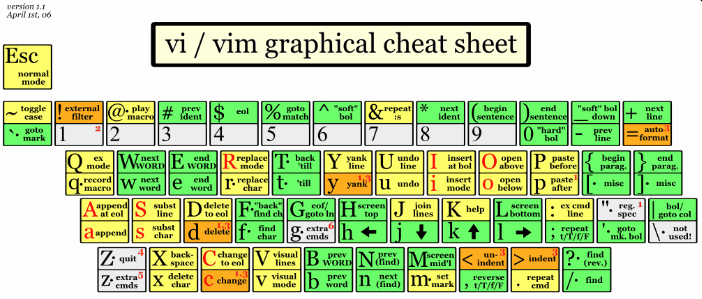
\includegraphics[width=230px]{images/vim-cheat-sheet.png}}
		\end{column}
	\end{columns}
\end{frame}
\begin{frame}{hjkl - Enkel navigasjon (normal) og redigering (insert)}
	\begin{center}
		\begin{itemize}
			\item h,j,k,l $\rightarrow$ Flytt som piltastene
			\item w, b, e $\rightarrow$ Flytt ordvis
			\item 0,\$ $\rightarrow$ Start og slutt av linje
			\item $<$C-d$>$, $<$C-u$>$, zz $\rightarrow$ Scrolling
			\item i,I,A $\rightarrow$ Insert mode
			\item $<$Esc$>$ $\rightarrow$ Normal mode
		\end{itemize}
		{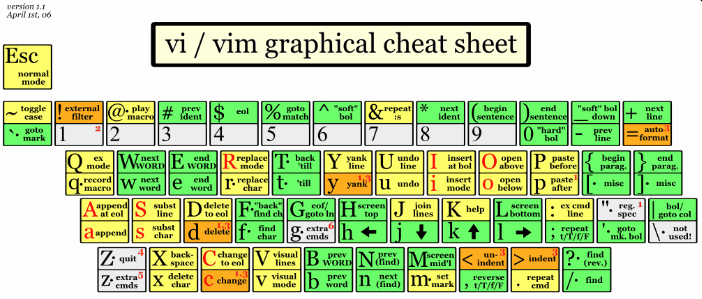
\includegraphics[width=230px]{images/vim-cheat-sheet.png}}
	\end{center}
\end{frame}

\begin{frame}{Vim som et språk med operatorer}
	\begin{center}
		\begin{columns}
			\begin{column}{0.5\textwidth}
				\begin{itemize}
					\item Operatorer
					      \begin{itemize}
						      \item Change (c + motion)
						      \item Delete (d + motion)
						      \item Yank (y + motion, copy)
					      \end{itemize}
				\end{itemize}
			\end{column}
			\begin{column}{0.5\textwidth}
				\begin{itemize}
					\item Motions
					      \begin{itemize}
						      \item Alle måter å bevege seg på
						      \item iw $\rightarrow$ inside word
						      \item i) $\rightarrow$ inside ()
                              \item f$\{$char$\}$ → Til char
					      \end{itemize}
				\end{itemize}
			\end{column}
		\end{columns}
		\vspace{20px}
		Derfor: ci) $\rightarrow$ change inside ()
		{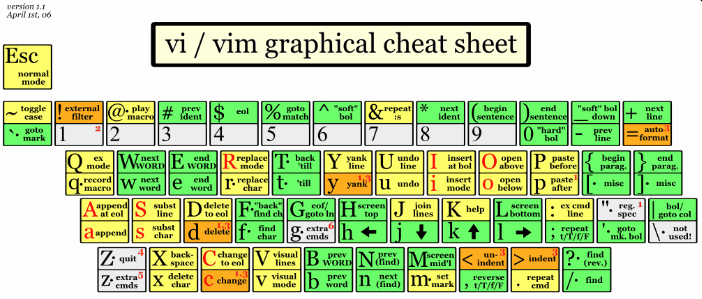
\includegraphics[width=230px]{images/vim-cheat-sheet.png}}
	\end{center}
\end{frame}

\begin{frame}{Litt mer avansert redigering}
    \begin{itemize}
        \item Marks - Husk en posisjon i filen
        \item Registers - Lagre i clipboard
        \item Makroer - Lagre en sekvens av kommandoer
    \end{itemize}
\end{frame}

\begin{frame}{Kult konsept, men jeg liker ikke terminalen...}
	\begin{itemize}
		\item Omtrent alle store editorer har en Vim plugin/extension
		      \begin{itemize}
			      \item VSCode
			      \item IntelliJ
			      \item Emacs
			      \item Atom
			      \item Chrome/Firefox
			      \item Zathura (PDF)
			      \item Mange flere
		      \end{itemize}
	\end{itemize}
\end{frame}

\begin{frame}{Konfigurer Neovim til å bli en IDE}
	\begin{itemize}
		\item Vimscript/Lua konfigurasjon
		\item LSP
		\item Treesitter
		\item Must-have plugins
        \item Neovim only
	\end{itemize}
\end{frame}

\begin{frame}{Lua konfigurasjon}
	\begin{itemize}
		\item Lua $\approx$ Python
		\item Nytt innebygd språk i Neovim
		\item Konfigurere Neovim → init.lua
		\item Vimscript finnes, legacy
	\end{itemize}
\end{frame}


\begin{frame}{LSP}
	\begin{itemize}
		\item Kjør en ``Language-server`` i bakgrunnen
		\item Tilbyr:
		      \begin{itemize}
			      \item Auto-completion
			      \item Go-to-definition
			      \item Rename variable
			      \item Diverse Code-actions
			      \item Utrolig mye mer
		      \end{itemize}
	\end{itemize}
\end{frame}


\begin{frame}{Treesitter}
\begin{itemize}
    \item Parser generator som genererer raske incremental parsere
    \item Syntax-highlighting, refaktorering, søking
    \item Stort potensiale for plugins
\end{itemize}

\end{frame}

\begin{frame}{``Must-have`` plugins}
	\begin{itemize}
		\item nvim-cmp (Auto-completion)
		\item Telescope (Fuzzy-finder)
		\item vim-fugitive (Git)
        \item Which-key (Mappings)
		\item Neorg (Notater)
        \item Flere: \url{https://github.com/rockerBOO/awesome-neovim}
	\end{itemize}
\end{frame}

\begin{frame}{Min workflow}
    \begin{itemize}
        \item Finne mapper/filer/kode - Telescope
        \item Bevegelse
            \begin{itemize}
                \item Scrolling - $<$C-u$>$/$<$C-d$>$ 
                \item Vertikal bevegelse - $\{$count$\}$j/k med mappings
                \item Horisontal bevegelse - f/t$\{$char$\}$
                \item Større bevegelser - Søk med $/$
            \end{itemize}
        \item Alle andre convenient mappings - Which-key
    \end{itemize}
\end{frame}

\begin{frame}{Siste tips}
    \begin{itemize}
        \item Prøv Vim i hvertfall 2-4 uker
        \item Map Caps lock til Escape
        \item Vimtutor / Vim-adventures
        \item Pre-made konfigurasjoner (LunarVim)
    \end{itemize}
\end{frame}
\begin{frame}{Takk for meg!}
    \begin{itemize}
        \item \url{https://www.vim.org/}
        \item \url{https://neovim.io/}
        \item \url{https://github.com/LunarVim/LunarVim}
        \item \url{https://github.com/jakobkhansen/dotfiles/}
        \item \url{https://github.com/jakobkhansen/VimTalk}
    \end{itemize}
    :wq
\end{frame}

\begin{frame}
\end{frame}


\end{document}
